% Interview presentation of the collaborative Pi Durable fork.
% Build: python build.py --moloch-source E:/Github/moloch --tectonic <tectonic.exe>
% Speaker notes come from notes.json; build.py emits notes.generated.tex privately.
\documentclass[11pt,aspectratio=169]{beamer}
\usetheme[progressbar=frametitle,sectionpage=none]{moloch}
\usepackage{booktabs}
\usepackage{array}
\usepackage{lmodern}
\usepackage{pgfpages}
\setbeamertemplate{navigation symbols}{}
\setbeamertemplate{page number in head/foot}[framenumber]
\setbeamersize{text margin left=9mm,text margin right=9mm}
\setbeamerfont{title}{size=\LARGE,series=\bfseries}
\setbeamerfont{frametitle}{size=\large,series=\bfseries}
\setbeamerfont{note page}{size=\small}
\setlength{\tabcolsep}{5pt}
\renewcommand{\arraystretch}{1.3}
\newcolumntype{L}[1]{>{\raggedright\arraybackslash}p{#1}}
\hypersetup{pdftitle={Collaborative Pi Durable},pdfauthor={Take-home project}}
\newcommand{\keypoint}[1]{\par\medskip{\usebeamercolor[fg]{alerted text}\bfseries #1}\par}
\newcommand{\captionline}[1]{\par\medskip{\small #1}\par}
\input{notes.generated.tex}
\ifdefined\WithNotes
  \setbeameroption{show notes}
\else
  \setbeameroption{hide notes}
\fi
\title{Collaborative Pi Durable}
\subtitle{Multiple users, shared agents, one workspace}
\author{Engineering take-home}
\date{November 2026}


\begin{document}

% 01 -- Collaborative Pi Durable
\begin{frame}[plain]
  \titlepage
  \DeckNote{1}
\end{frame}

% 02 -- Two people share the same agent history
\begin{frame}{Two people share the same agent history}
  \begin{tabular}{@{}L{.21\textwidth}L{.33\textwidth}L{.37\textwidth}@{}}
    \toprule
    Person / agent & Instruction & Shared behavior \\
    \midrule
    Alice $\rightarrow$ OpenAI & Add a search box & Bob sees Alice's instruction \\
    Bob $\rightarrow$ OpenAI & Handle empty searches too & Same conversation and queue \\
    Bob $\rightarrow$ Ollama & Review the changed files & Same files; separate agent history \\
    \bottomrule
  \end{tabular}
  \captionline{Either user can stop a shared agent, including the other's queued work}
  \keypoint{The added requirement is coordination between people}
  \DeckNote{2}
\end{frame}

% 03 -- Demo: one person hands work to another
\begin{frame}{Demo: one person hands work to another}
  \centering
  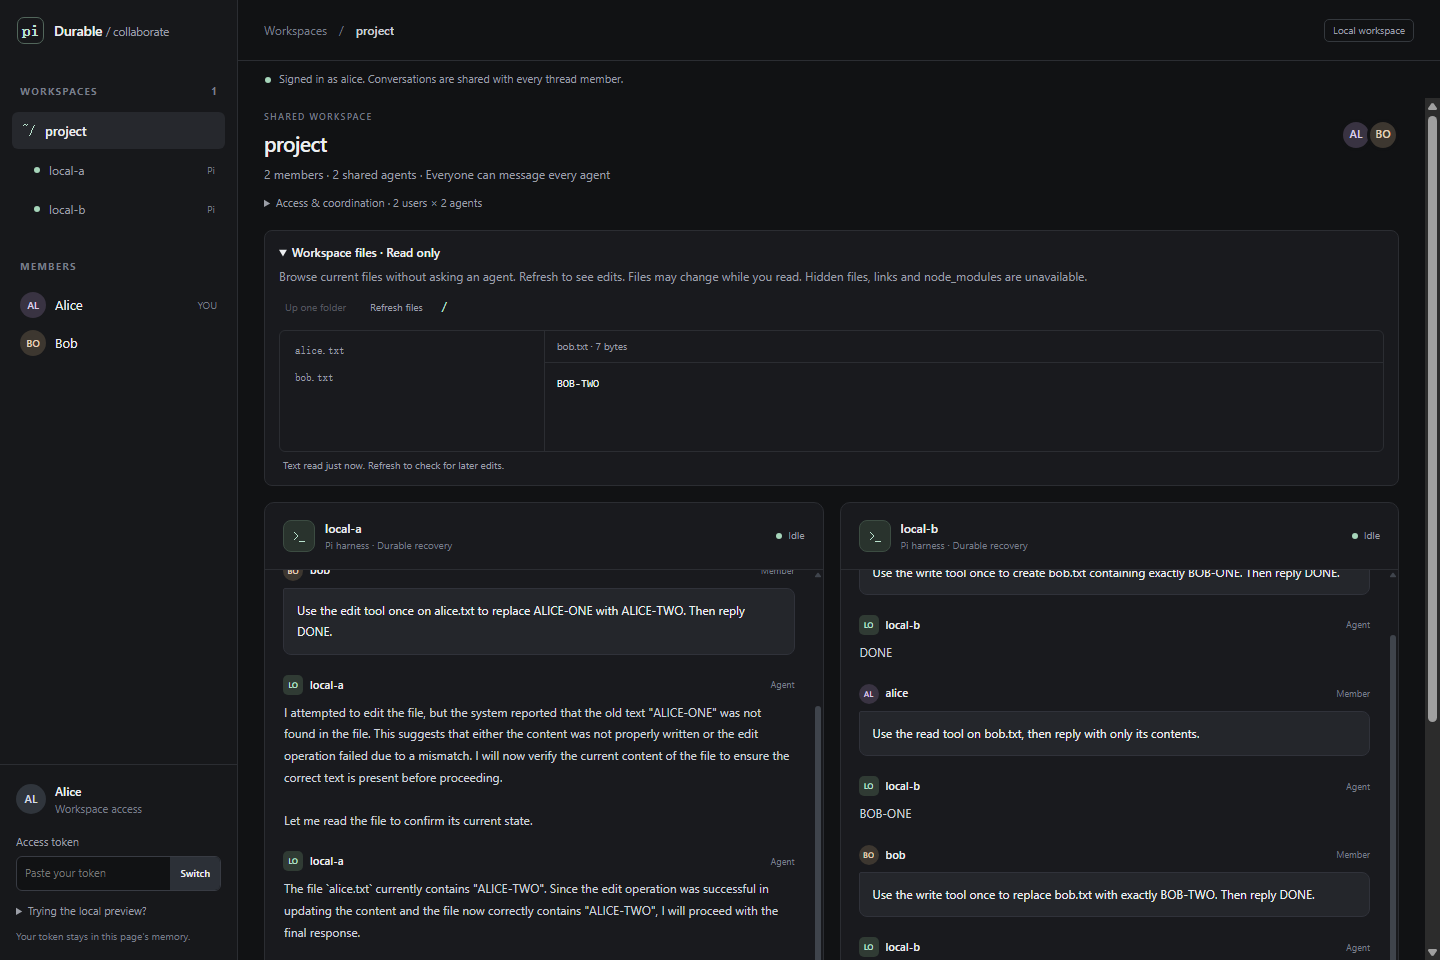
\includegraphics[height=.74\textheight]{assets/local-ollama-browser.png}
  \captionline{Recorded local Ollama run; live handoff uses Alice and Bob on the same agent}
  \DeckNote{3}
\end{frame}

% 04 -- Where the collaboration rules live
\begin{frame}{Where the collaboration rules live}
  \begin{tabular}{@{}p{.27\textwidth}p{.66\textwidth}@{}}
    \toprule
    Layer & Responsibility \\
    \midrule
    Web host & Identify the user; deliver commands and live views \\
    Collaboration package & Check membership; save requests with their authors \\
    Existing Durable & Run the model/tool loop; save state; recover work \\
    Execution paths & Pi AI model services, or a connector to the Codex app \\
    \bottomrule
  \end{tabular}
  \captionline{One owning runtime, SQLite store, and shared workspace per thread}
  \keypoint{Reuse the runtime; avoid a second web-owned execution queue}
  \DeckNote{4}
\end{frame}

% 05 -- Saving a request is separate from its answer
\begin{frame}{Saving a request is separate from its answer}
  \begin{enumerate}
    \item Save the instruction and the work together
    \item Acknowledge acceptance; run when the agent is ready
    \item Show progress and the eventual result
  \end{enumerate}
  \medskip
  \begin{tabular}{@{}L{.43\textwidth}L{.48\textwidth}@{}}
    \toprule
    Browser action & Server behavior \\
    \midrule
    Retry original ID + text & Find the saved request; no second command \\
    New Send with the same text & New ID; another command \\
    \bottomrule
  \end{tabular}
  \keypoint{Accepted $\neq$ completed $\neq$ correct file changes}
  \DeckNote{5}
\end{frame}

% 06 -- Activity shows requests, tools and current files
\begin{frame}{Activity shows requests, tools and current files}
  \begin{tabular}{@{}p{.27\textwidth}p{.66\textwidth}@{}}
    \toprule
    Observation & What the user can conclude \\
    \midrule
    Saved request / author & Who submitted; observed queue/run outcome \\
    Tool request / result & An operation was requested or returned a result \\
    Current file bytes & What is on disk when inspected \\
    \bottomrule
  \end{tabular}
  \captionline{Bounded recent evidence; reconnect may omit intermediate transitions}
  \keypoint{A completed tool does not prove the requested code is correct}
  \DeckNote{6}
\end{frame}

% 07 -- The stale-edit problem
\begin{frame}{The stale-edit problem}
  \begin{tabular}{@{}cp{.56\textwidth}l@{}}
    \toprule
    No. & Operation & File content \\
    \midrule
    1 & A and B both read the file & \texttt{base} \\
    2 & A writes its replacement & \texttt{base + alice} \\
    3 & B writes from its old copy & \texttt{base + bob} \\
    \bottomrule
  \end{tabular}\par
  \medskip
  Both commands can finish. Alice's change is gone.
  \captionline{A changed dependency can also invalidate an edit to an unchanged file}\keypoint{Taking turns at the final write does not fix an outdated read}
  \DeckNote{7}
\end{frame}

% 08 -- Demo: generate, publish, resolve and reset
\begin{frame}{Demo: generate, publish, resolve and reset}
  \begin{tabular}{@{}L{.25\textwidth}L{.34\textwidth}L{.32\textwidth}@{}}
    \toprule
    Action & Content & Outcome \\
    \midrule
    Both generate & Alice: Hello/light; Bob: Hi/dark & File stays Welcome/neutral \\
    Alice publishes & Hello/light & Applied \\
    Bob publishes & Hi/dark; old base & Refused; proposal retained \\
    User resolves & Chooses Hello/dark & Published after review \\
    \bottomrule
  \end{tabular}
  \captionline{Examples show greeting/theme. Reset starts a fresh shared round.}
  \keypoint{This check protects managed proposals; ordinary coding writes bypass it}
  \DeckNote{8}
\end{frame}

% 09 -- Agents know peers may change files
\begin{frame}{Agents know peers may change files}
  \textbf{Ollama writes blue $\rightarrow$ GPT changes it to green}
  \begin{itemize}
    \item Fresh context: peers may change the same files
    \item Reread, preserve unrelated edits, ask about conflicting intent
    \item Participant names and recent request references; no peer transcript
  \end{itemize}
  \captionline{Durable agents: before each model request. Codex: at turn open/resume.}
  \captionline{Extra input tokens, no extra model call; overhead not yet measured}
  \keypoint{Awareness helps reasoning; it does not enforce a safe write}
  \DeckNote{9}
\end{frame}

% 10 -- What survives a crash
\begin{frame}{What survives a crash}
  \textbf{Failure trace}\quad File changes $\rightarrow$ host dies $\rightarrow$ result not saved
  \medskip
  \begin{tabular}{@{}p{.33\textwidth}p{.60\textwidth}@{}}
    \toprule
    Action & Recovery behavior \\
    \midrule
    Same request ID/text & Find its saved request \\
    Durable model request & May repeat under Durable's recovery rules \\
    Uncertain Codex attempt & Mark interrupted; do not resend automatically \\
    Existing file changes & May remain; cancellation does not undo them \\
    \bottomrule
  \end{tabular}
  \keypoint{SQLite state and workspace writes are separate operations}
  \DeckNote{10}
\end{frame}

% 11 -- A model service versus an agent application
\begin{frame}{A model service versus an agent application}
  \begin{columns}[T,onlytextwidth]
    \begin{column}{.46\textwidth}
      \textbf{OpenAI / Ollama}
      \begin{itemize}
        \item Supply model output to Pi
        \item Durable runs the tool loop
        \item Current default: both providers
      \end{itemize}
    \end{column}
    \begin{column}{.48\textwidth}
      \textbf{Codex application}
      \begin{itemize}
        \item Runs its own model/tool loop
        \item T3 code connects it to Durable
        \item Real coding turn still unverified
      \end{itemize}
    \end{column}
  \end{columns}
  \keypoint{A second model service is different from a second agent application}
  \DeckNote{11}
\end{frame}

% 12 -- What our checks establish
\begin{frame}{What our checks establish}
  \begin{tabular}{@{}p{.25\textwidth}p{.68\textwidth}@{}}
    \toprule
    Test type & What it establishes \\
    \midrule
    Controlled scenarios & Retry rules, ordering, lost updates, selected crash boundaries \\
    Real local model & Actual tool calls, file bytes, shared browser state, idle reopen \\
    Simulated load & Real HTTP/SSE and SQLite; 1,200 commands over about 10 minutes \\
    \bottomrule
  \end{tabular}
  \captionline{Burst: 81 accepted/completed; 519 rejected at configured capacity}
  \keypoint{The first observed limit was the queue cap, not maximum throughput}
  \DeckNote{12}
\end{frame}

% 13 -- GCP deployment and remaining checks
\begin{frame}{GCP deployment and remaining checks}
  \textbf{Browser $\rightarrow$ sslip.io address $\rightarrow$ Caddy $\rightarrow$ app}
  \begin{itemize}
    \item One VM owns the saved state and workspace
    \item Cloud website accessible; verify the latest deployed revision
    \item Slow GCP Ollama chat remains under investigation
    \item Verify the deployed revision, cleanup and backup restoration
  \end{itemize}
  \keypoint{A reachable website does not establish reliable recovery or latency}
  \DeckNote{13}
\end{frame}

% 14 -- What is implemented and what comes next
\begin{frame}{What is implemented and what comes next}
  \textbf{Implemented}
  \begin{itemize}
    \item Shared users/agents, saved requests and visible activity
    \item Peer awareness; managed generate/publish/resolve/reset
  \end{itemize}
  \medskip
  \textbf{Next protection and delivery work}
  \begin{itemize}
    \item Managed coding tools and dependency-version checks
    \item GCP latency/rehearsal, real Codex turns and restore checks
  \end{itemize}
  \keypoint{The controlled proposal flow is narrower than general coding safety}
  \DeckNote{14}
\end{frame}

\appendix

% 15 -- Backup: file protection and dependencies
\begin{frame}{Backup: file protection and dependencies}
  \begin{tabular}{@{}L{.24\textwidth}L{.33\textwidth}L{.33\textwidth}@{}}
    \toprule
    Choice & Benefit & Cost / limit \\
    \midrule
    Destination check & Refuse an outdated replacement & Current managed file only \\
    Dependency checks & Detect changes to files the plan used & Future: track reads; coordinate publication \\
    Whole-task ownership & Keep participating writers apart & Less overlap; stop all child writers \\
    Separate worktrees & Isolate edits in different directories & Review, merge and test later \\
    \bottomrule
  \end{tabular}
  \DeckNote{15}
\end{frame}

% 16 -- Backup: trusted users and shared control
\begin{frame}{Backup: trusted users and shared control}
  \begin{itemize}
    \item Host authenticates; package checks membership
    \item All members can inspect and stop all agent lanes
    \item A workspace path is not an operating-system sandbox
    \item Queue limits do not establish fairness or a spending limit
  \end{itemize}
  \keypoint{Trusted collaborators, fixed configuration, one owner}
  \DeckNote{16}
\end{frame}

% 17 -- Backup: reconnect and request retries
\begin{frame}{Backup: reconnect and request retries}
  \begin{itemize}
    \item HTTP sends commands; SSE delivers current-state views
    \item Reconnect fetches recent state; older history is paged
    \item Slow viewers keep a latest pending snapshot
    \item No promise to replay every token or a global audit log
  \end{itemize}
  \keypoint{Browser reload can lose an ambiguous request's local retry ID}
  \DeckNote{17}
\end{frame}

% 18 -- Backup: design choices and AI assistance
\begin{frame}{Backup: design choices and AI assistance}
  \textbf{Decisions I can explain}
  \begin{itemize}
    \item Extend Durable rather than add a second runtime
    \item Require actual T3 reuse; keep adapter details separate
    \item Distinguish duplicate requests from duplicate effects
    \item Test actual files and expose remaining conflict risks
  \end{itemize}
  \captionline{AI assisted implementation and documentation; upstream code is credited}
  \DeckNote{18}
\end{frame}

\end{document}
